\documentclass{scrartcl}
\usepackage[utf8]{inputenc}
\usepackage{tikz}
\usetikzlibrary{arrows,decorations.pathmorphing,backgrounds,fit,positioning,shapes.symbols,chains,shapes.geometric,shapes.arrows,calc}

\begin{document}
 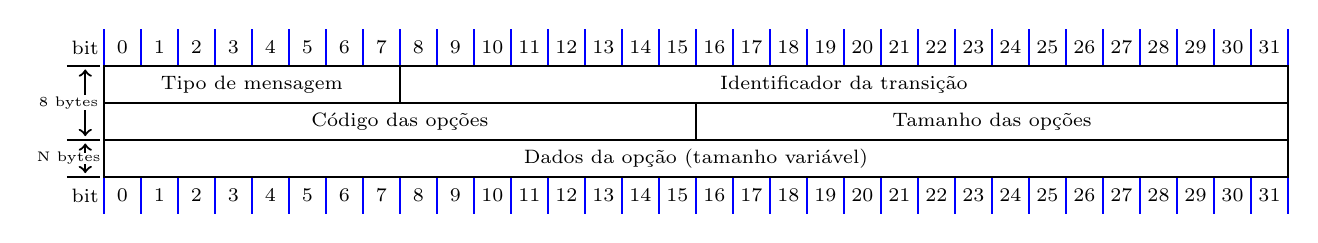
\begin{tikzpicture}[scale=0.47]
\foreach \x in {0,...,31}
\node at (\x+0.5,20.5) {\scriptsize \x};
\foreach \x in {0,...,31}
\node at (\x+0.5,16.5) {\scriptsize \x};
\foreach \x in {0,...,32}
\draw[thick, blue] (\x,16) -- (\x,21);
\node[thick] (bit1) at (-0.5,20.5) {\scriptsize bit};
\node[thick] (bit2) at (-0.5,16.5) {\scriptsize bit};
\draw [<->, thick] (-0.5, 19.9) -- (-0.5,18.1);
%\draw [<->, thick] (-0.5, 18.9) -- (-0.5,18.1);
\draw [<->, thick] (-0.5, 17.9) -- (-0.5,17.1);
\draw [thick] (-1, 20) -- (-0.1,20);
%\draw [thick] (-1, 19) -- (-0.1,19);
\draw [thick] (-1, 18) -- (-0.1,18);
\draw [thick] (-1, 17) -- (-0.1,17);
\fill[white] (-0.8,19.2) rectangle (-0.1,18.8);
%\fill[white] (-0.8,18.65) rectangle (-0.1,18.35);
\fill[white] (-0.8,17.65) rectangle (-0.1,17.35);
\node at (-0.95,19) {\tiny 8 bytes};
\node at (-0.95,17.5) {\tiny N bytes};
\filldraw[thick,draw=black, fill=white] (0,20) rectangle (8,19); \node (mode) at (4,19.5) {\scriptsize Tipo de mensagem};
\draw[thick, draw=black, fill=white] (8,20) rectangle (32,19); \node (li) at (20,19.5) {\scriptsize Identificador da transição};
%\draw[thick, draw=black, fill=white] (16,20) rectangle (32,19); \node (li) at (24,19.5) {\scriptsize \textit{Checksum}};
\filldraw[thick,draw=black, fill=white] (0,19) rectangle (16,18); \node (mode) at (8,18.5) {\scriptsize Código das opções};
\draw[thick, draw=black, fill=white] (16,19) rectangle (32,18); \node (li) at (24,18.5) {\scriptsize Tamanho das opções};
\filldraw[thick,draw=black, fill=white] (0,18) rectangle (32,17); \node (mode) at (16,17.5) {\scriptsize Dados da opção (tamanho variável)};
\end{tikzpicture}	\end{tikzpicture}
\end{document}
